\documentclass[11pt,a4paper]{article}

\usepackage{amsmath}
\usepackage{amsfonts}
\usepackage{amssymb}
\usepackage{graphicx}
\usepackage[left=1in,right=1in,top=1in,bottom=1in]{geometry}

\title{Machine Learning in Complex Domains:\\Assignment 3}
\author{Ryan Cotterell, Daniel Deutsch, Dan Crankshaw}
\date{}

\begin{document}

	\maketitle
	
	\setcounter{section}{3}
	\section{Blocked Gibbs Sampler}
	
	\subsection{Analysis Questions}


        We have the following equation
$$
p(z_{d,i} = k,x_{d,i} = c| \mathbf{z} - z_{d,i},\mathbf{x} - x_{d,i}, \mathbf{c},\mathbf{w} ; \alpha,\beta,\lambda) = \frac{p(\mathbf{z},\mathbf{x},\mathbf{c},\mathbf{w}|\alpha,\beta,\lambda)}{p(\mathbf{z} - z_{d,i},\mathbf{x} - x_{d,i},\mathbf{c},\mathbf{w} ; \alpha,\beta,\lambda)}
$$
The full join (numerator) is given to us in the assignment. We can factor this according to the joint and every term that does not involve $z_{d,i}$ or $x_{d,i}$ will cancel. This is basically a union of (15) and (18). This yields the following:
$$
p(z_{d,i} = k, x_{d,i} = 0| \mathbf{z} - z_{d,i},\mathbf{x} - x_{d,i}, \mathbf{c},\mathbf{w} ; \alpha,\beta,\lambda) = \frac{p(x=0|\lambda)
  \frac{\Gamma(n^k_{w_{d,i}} + 1 + \beta)}{\Gamma(1 + \sum_w n_w^k + \beta )} 
    \frac{\Gamma(n_k^d + 1 + \alpha)}{\Gamma(1 + \sum_{k'} n_{k'}^d + \alpha)}
    }
    {
    \frac{\Gamma(n_{w_{d,i}}^k + \beta)}{\Gamma(\sum_w n_w^k + \beta )}
    \frac{\Gamma(n_k^d + \alpha)}{\Gamma(\sum_{k'} n_{k'}^d + \alpha) } 
    }
$$
$$
p(z_{d,i} = k, x_{d,i} = 0| \mathbf{z} - z_{d,i},\mathbf{x} - x_{d,i}, \mathbf{c},\mathbf{w} ; \alpha,\beta,\lambda) \propto \frac{(1-\lambda) (n_{w_{d,i}}^k + \beta) (n_k^d + \alpha)}{(n_*^k + K\beta)(n_*^d + V\alpha)}
$$
By analogy, we get the followoing for the case that $p(x=1)$. 
$$
p(z_{d,i} = k, x_{d,i} = 1| \mathbf{z} - z_{d,i},\mathbf{x} - x_{d,i}, \mathbf{c},\mathbf{w} ; \alpha,\beta,\lambda) \propto \frac{\lambda (n_{w_{d,i}}^k + \beta) (n_k^d + \alpha)}{(n_*^k + K\beta)(n_*^d + V\alpha)}
$$
Most of the heavy lifting for this question was done in the appendix so there isn't really any more we can write. 

	
	\section{Text Analysis with MCLDA}
	\subsection{Empirical Questions}
	\begin{enumerate}
		\item
			\begin{figure}[h]
				\begin{center}
					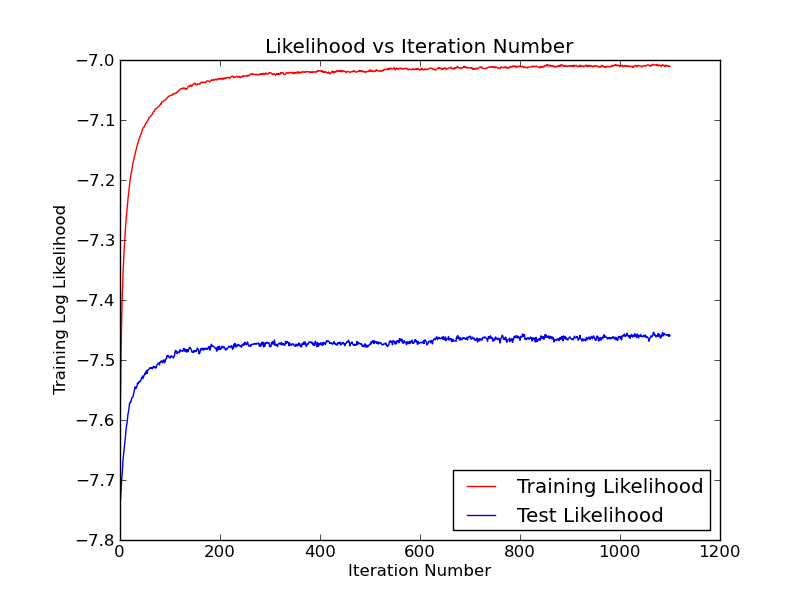
\includegraphics[scale=0.5]{../train_test_1}
				\end{center}
			\end{figure}
			\begin{figure}[h]
				\begin{center}
					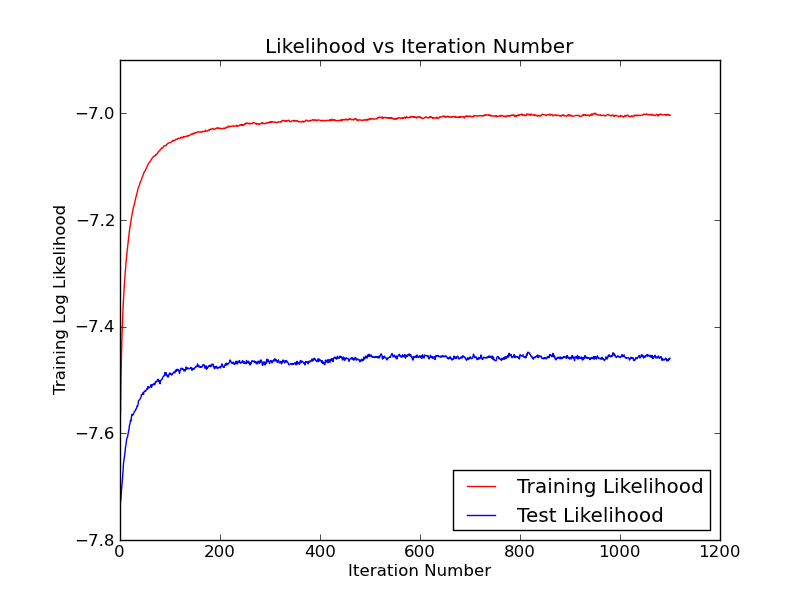
\includegraphics[scale=0.5]{../train_test_2}
				\end{center}
			\end{figure}
			\begin{figure}[h]
				\begin{center}
					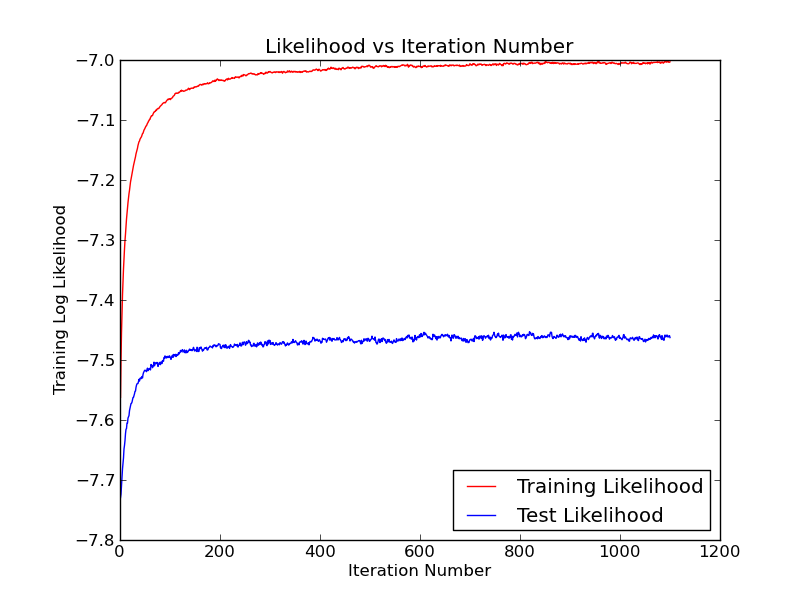
\includegraphics[scale=0.5]{../train_test_3}
				\end{center}
			\end{figure}
		\item 
			\begin{figure}[h]
				\begin{center}
					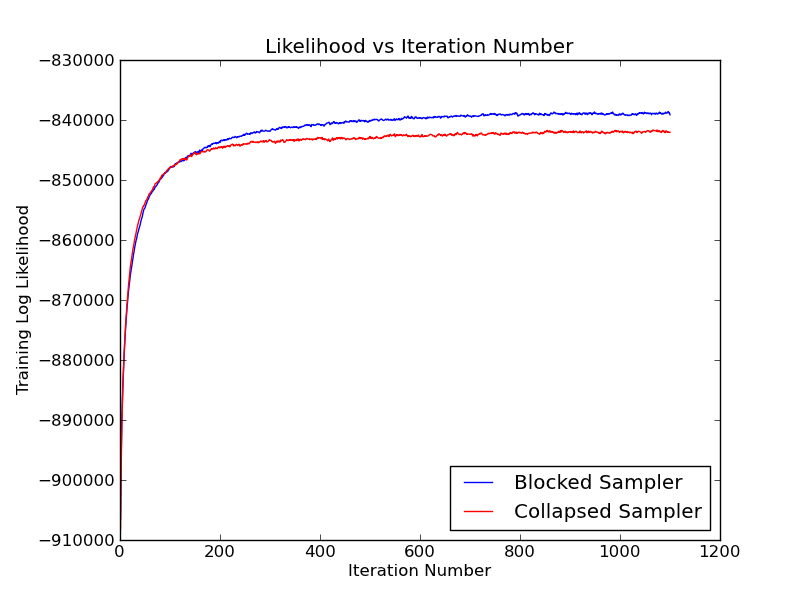
\includegraphics[scale=0.5]{../block_v_collapse_plot}
				\end{center}
			\end{figure}
		\item
			\begin{figure}[h]
				\begin{center}
					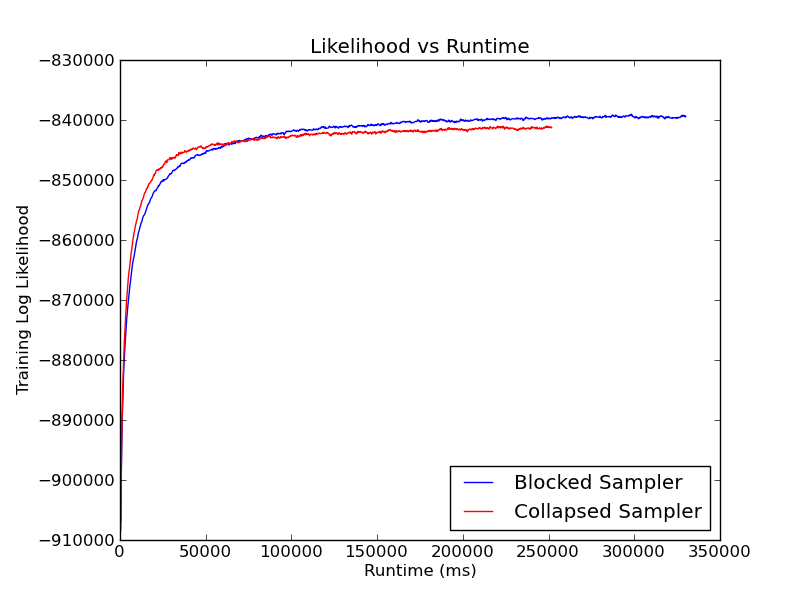
\includegraphics[scale=0.5]{../runtime_plot}
				\end{center}
			\end{figure}
		\item
			\begin{figure}[h]
				\begin{center}
					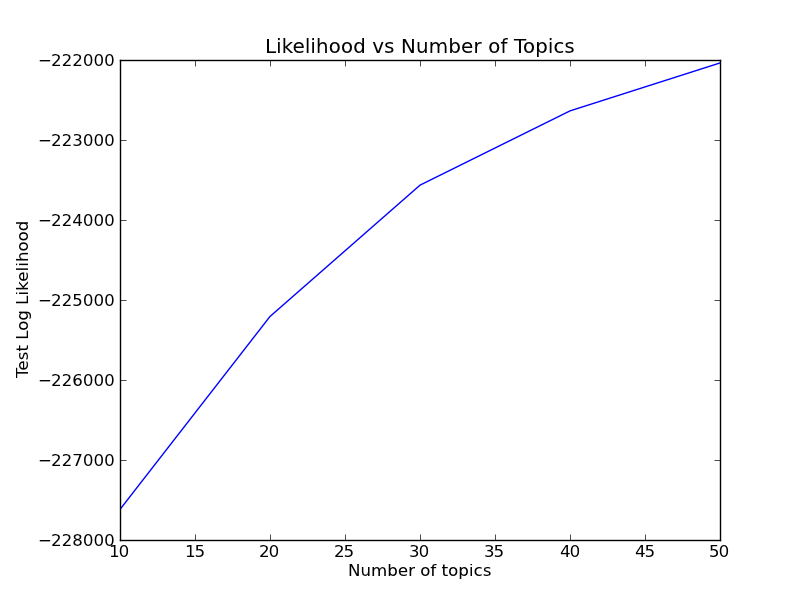
\includegraphics[scale=0.5]{../topics_plot}
				\end{center}
			\end{figure}
		\item
			\begin{figure}[h]
				\begin{center}
					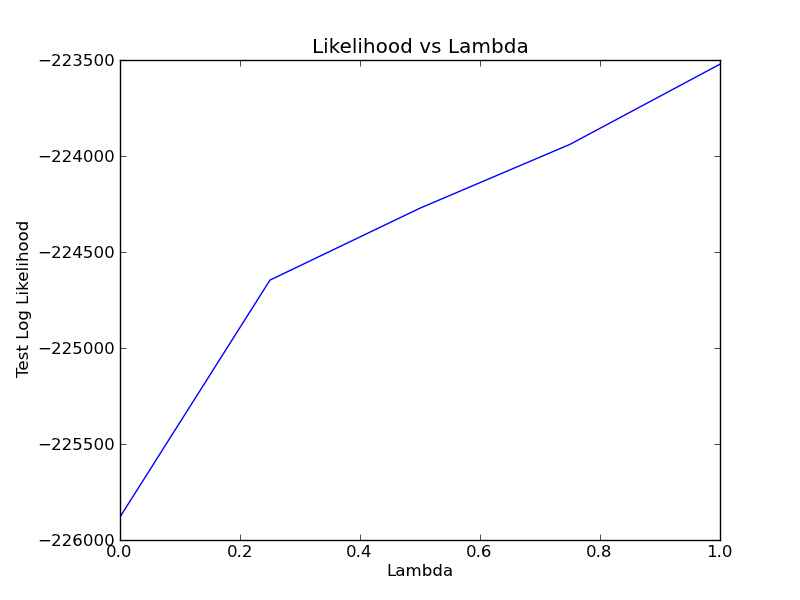
\includegraphics[scale=0.5]{../lambda_plot}
				\end{center}
			\end{figure}
		\item \begin{enumerate}
			\item 
			\item 
			\item 
		\end{enumerate}
	\end{enumerate}
	
	\section{Variational Inference}
	\subsection{Analysis Questions}
	
	\setcounter{subsection}{2}
	\subsection{Empirical Questions}
	\begin{enumerate}
		\item 
		\item
		\item
		\item
	\end{enumerate}

\end{document}
